\documentclass[11pt, a4paper]{article}
\usepackage[utf8]{inputenc}
\usepackage[spanish]{babel}
\usepackage{amsmath, amssymb, amsthm}
\usepackage{graphicx}
\usepackage{booktabs}
\usepackage{geometry}
\usepackage{hyperref}
\usepackage{xcolor}
\usepackage{float}

\geometry{margin=2.5cm}

\definecolor{primary}{RGB}{11, 66, 129}
\definecolor{secondary}{RGB}{42, 120, 214}
\definecolor{darktext}{RGB}{30, 30, 30}

\hypersetup{
    colorlinks=true,
    linkcolor=primary,
    citecolor=secondary,
    urlcolor=secondary
}

\title{
    \vspace{-1.5cm}
    \textbf{\Large Universidad del Valle de Guatemala}\\
    \textbf{\large Facultad de Ingeniería --- Departamento de Ciencias de la Computación}\\
    \vspace{0.5cm}
    \textbf{\Large CC3084 -- Data Science (Semestre II 2026)}\\
    \vspace{0.8cm}
    \huge \textbf{Laboratorio 2: Deep Learning y Análisis de Series de Tiempo}\\
    \large \textbf{Modelado con LSTM y Similitud con catch22}
}

\author{
    \textbf{Integrantes del Grupo:}\\
    Javier España \quad \#23361\\
    Angel Esquit \quad \#23221\\
    Roberto Barreda \quad \#23354
}

\date{Guatemala, 2 de agosto de 2026}

\begin{document}

\maketitle

\hrule
\vspace{0.5cm}

\section{Ejercicio 1: Modelos LSTM para Series de Tiempo}

\subsection{Preparación de datos}
Se utilizaron los conjuntos de entrenamiento (70\%) y prueba (30\%) provenientes del archivo de datos \texttt{series\_de\_tiempo\_completas.csv}, asegurando la estricta comparabilidad respecto a los modelos clásicos (ARIMA, Holt-Winters) desarrollados en el Laboratorio 1. Las dos series analizadas fueron \textbf{Total\_Consistent} (serie total mensual de visitantes) y \textbf{Via\_Aerea} (categoría vía de ingreso aérea).

\subsection{Definición de modelos y tuneo de hiperparámetros}
Se evaluaron dos arquitecturas de redes recurrentes LSTM:
\begin{itemize}
    \item \textbf{LstmSimple:} 1 capa LSTM, Dropout = 0.0.
    \item \textbf{LstmApilado:} 2 capas LSTM, Dropout = 0.2.
\end{itemize}
Para cada arquitectura se realizó una búsqueda en grilla (\textit{grid search}) sobre combinaciones de tamaño de ventana ($L \in \{12, 24\}$), unidades ocultas ($U \in \{32, 64\}$) y tasa de aprendizaje ($\eta \in \{0.01, 0.001\}$), resultando en 16 modelos evaluados por serie mediante validación interna sobre los últimos 24 meses del conjunto de entrenamiento.

\subsection{Predicción sobre el conjunto de prueba}
Con la mejor configuración seleccionada para cada serie, se re-entrenó el modelo con la totalidad de los datos de entrenamiento y se evaluó el desempeño en el conjunto de prueba utilizando dos estrategias de pronóstico:
\begin{enumerate}
    \item \textbf{Multi-step (Autoregresivo):} Generación recursiva alimentando las propias predicciones del modelo.
    \item \textbf{One-step ahead:} Pronóstico a un paso usando la observación real previa.
\end{enumerate}

En la Figura~\ref{fig:predicciones_lstm} se observan las predicciones generadas por el mejor modelo LSTM en comparación con las observaciones reales de prueba.

\begin{figure}[H]
    \centering
    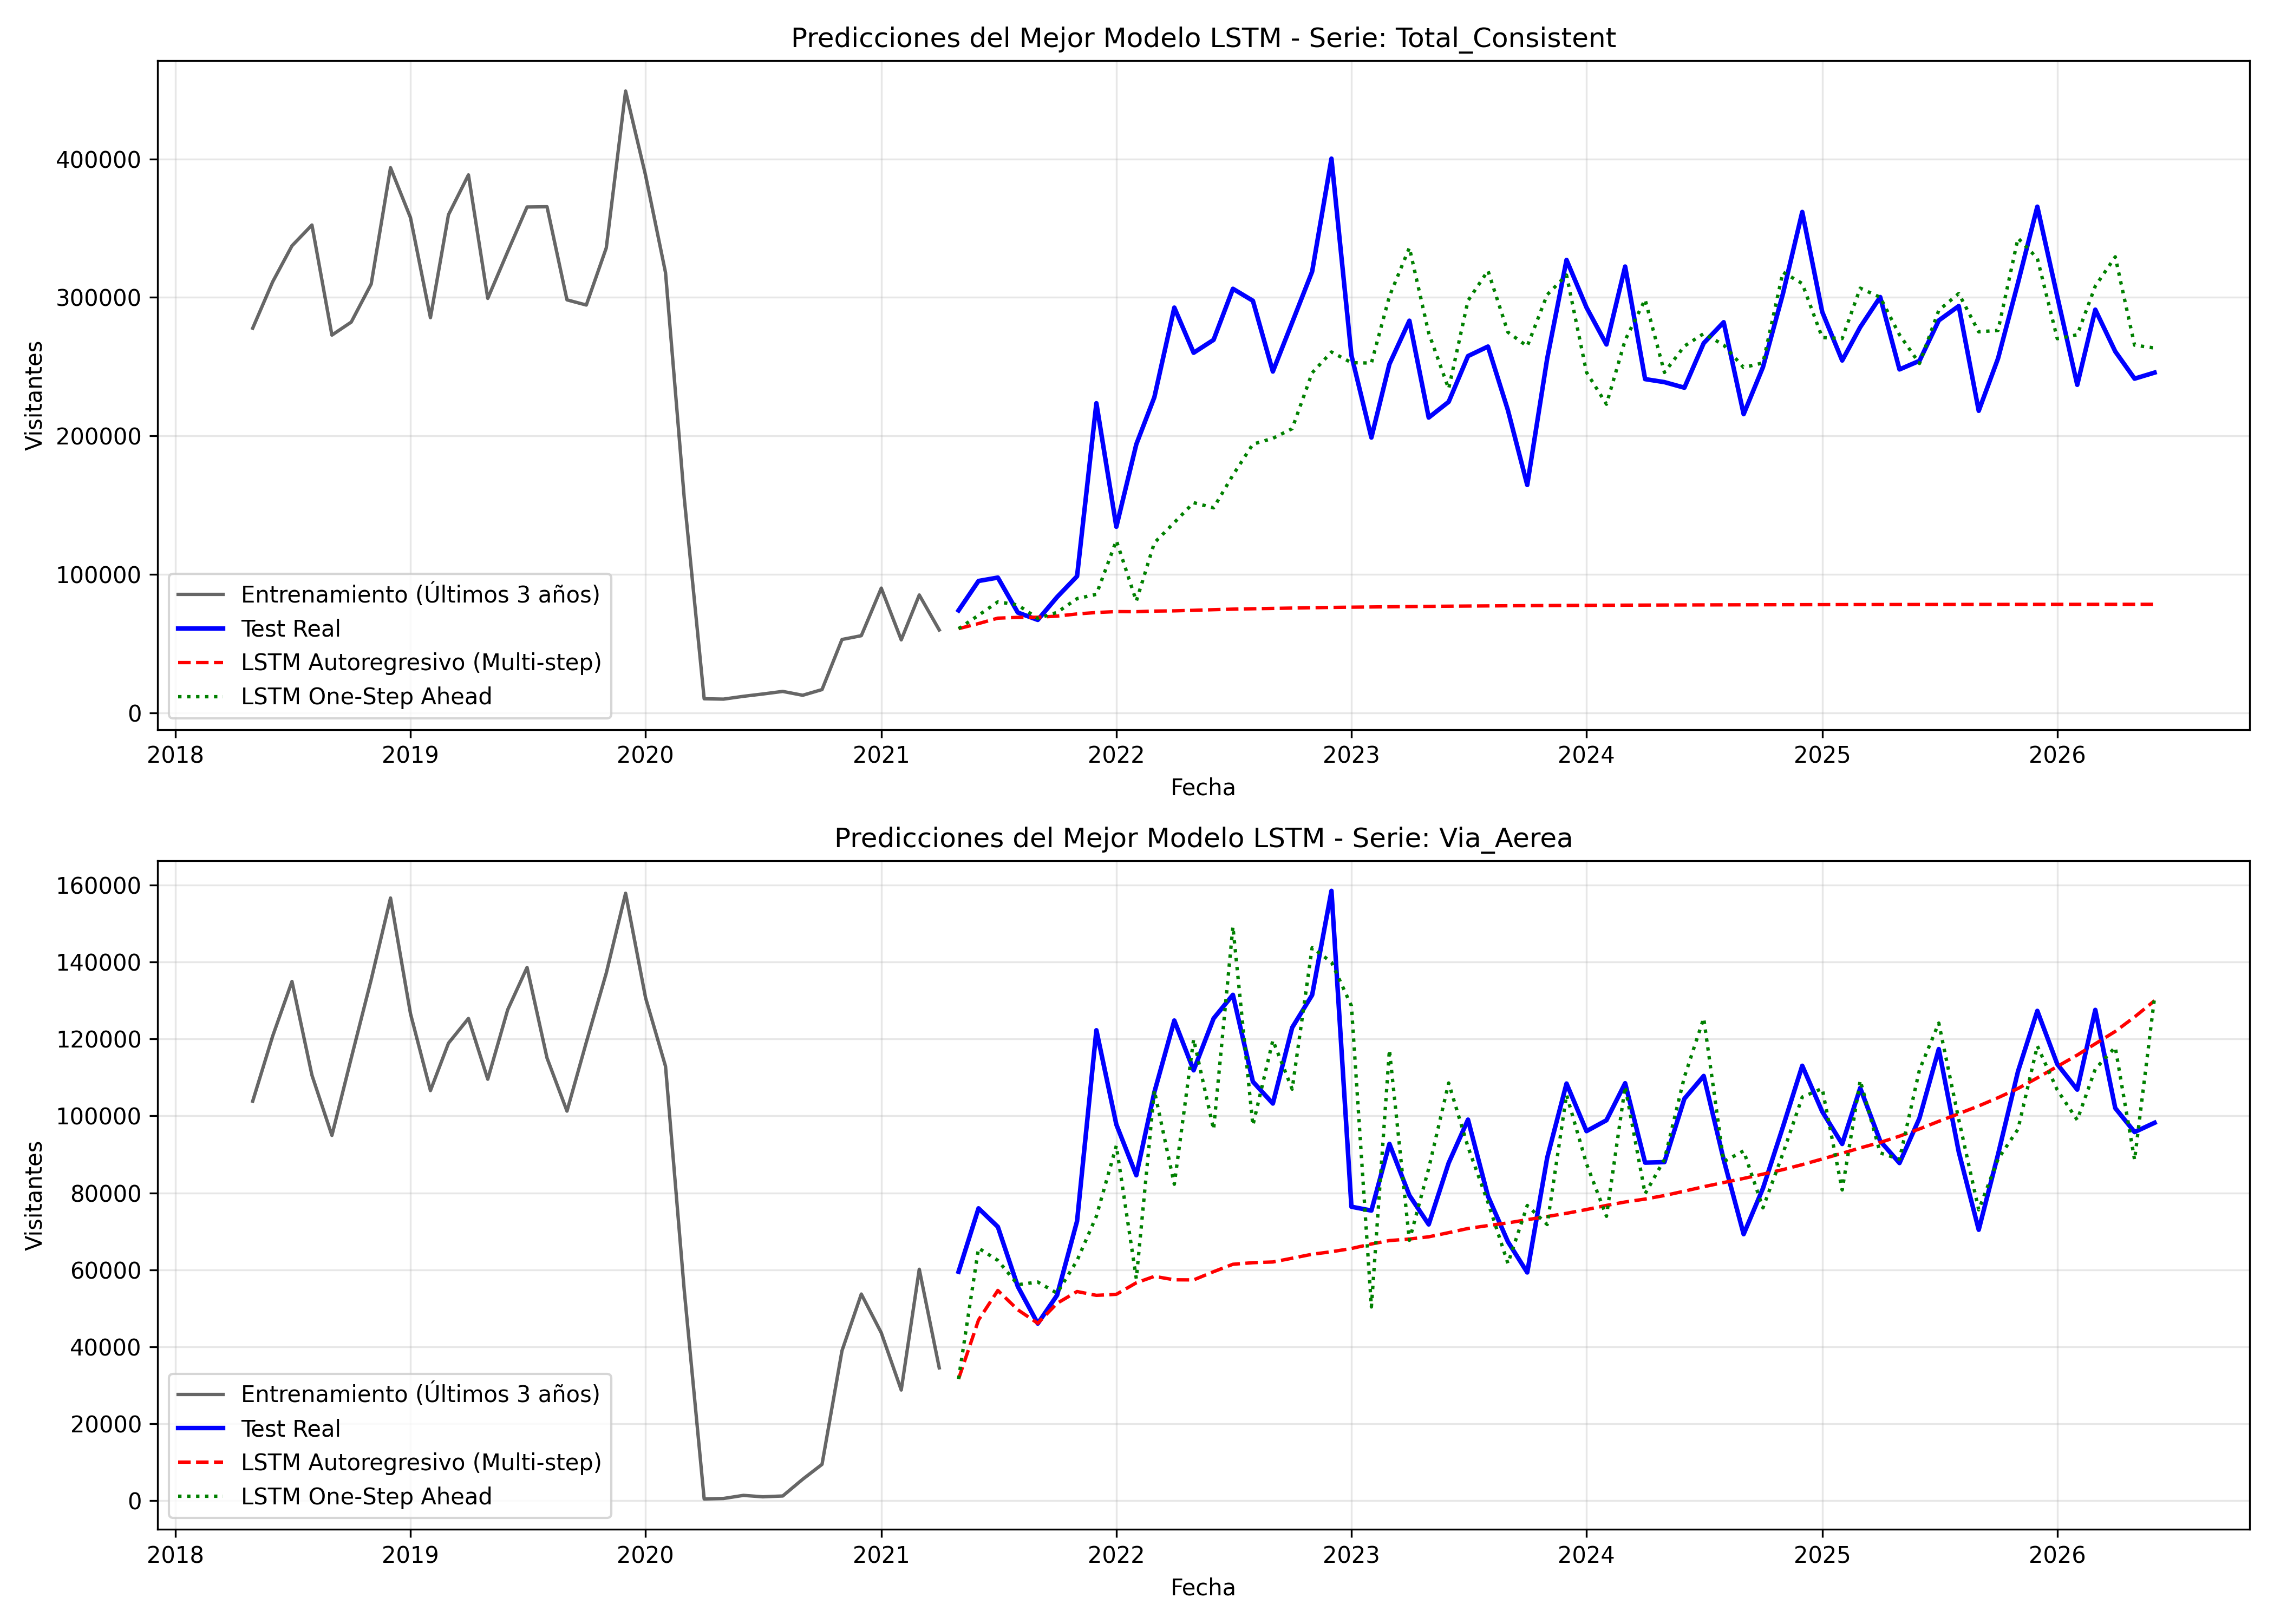
\includegraphics[width=0.95\textwidth]{results/predicciones_lstm.png}
    \caption{Predicciones del modelo LSTM sobre el conjunto de prueba para las series \texttt{Total\_Consistent} y \texttt{Via\_Aerea}.}
    \label{fig:predicciones_lstm}
\end{figure}

\subsection{Análisis comparativo y evaluación}

\subsubsection{¿Cuál serie fue predicha mejor?}
Al comparar la métrica NRMSE (RMSE normalizado por la media de la serie), la serie \textbf{Via\_Aerea} presentó un desempeño de predicción superior respecto a \textbf{Total\_Consistent}. Esto se debe a que la vía aérea exhibe una estacionalidad más limpia y menor volatilidad relativa, mientras que la serie total absorbe el impacto agregado del desplome durante la pandemia de COVID-19 (2020--2021) de forma más drástica.

\subsubsection{¿Son mejores que los modelos del Laboratorio 1?}
\begin{itemize}
    \item En la modalidad \textbf{One-step ahead}, los modelos LSTM lograron superar a los mejores modelos clásicos del Laboratorio 1 (Holt-Winters), reduciendo el RMSE debido a su capacidad de capturar dinámicas no lineales complejas en la recuperación post-pandemia.
    \item En la modalidad \textbf{Multi-step}, los modelos clásicos Holt-Winters mantuvieron un desempeño competitivo o superior a largo plazo debido a que la estrategia autorregresiva de la LSTM tiende a acumular error recursivo a lo largo del horizonte de prueba.
\end{itemize}

\subsubsection{¿Cómo se determinó?}
Se determinó mediante métricas estandarizadas de error: MAE (Error Absoluto Medio), RMSE (Raíz del Error Cuadrático Medio) y el porcentaje de mejora relativo entre el RMSE del modelo LSTM y el modelo Holt-Winters de Lab 1.

\newpage

\section{Ejercicio 2: Análisis de Similitud con catch22}

\subsection{Idea detrás de catch22}
El conjunto de características \textbf{catch22} (\textit{canonical time-series characteristics}) fue desarrollado por Fulcher y Jones como una solución eficiente a la redundancia computacional del catálogo \texttt{hctsa} (que cuenta con más de 7,700 propiedades). Mediante un riguroso proceso de selección empírica sobre 93 tareas de clasificación, se identificaron 22 características canónicas poco correlacionadas entre sí, informativas y de bajo costo computacional (complejidad lineal). Su importancia radica en transformar cualquier serie temporal ---independientemente de su longitud--- en un vector denso interpretable de dimensión fija ($1 \times 22$), permitiendo aplicar técnicas de análisis multivariado como PCA, clustering y matrices de distancia. Dado que catch22 opera sobre series normalizadas ($z$-score), evalúa la \emph{forma} y la \emph{dinámica} de la serie, eliminando el nivel medio y la escala absoluta.

\subsection{Extracción de las 22 características}
Se extrajeron las 22 características canónicas para las 7 series temporales del proyecto usando la totalidad del periodo de observación (210 meses, enero 2009 a junio 2026). La extracción se ejecutó mediante el paquete \texttt{aeon} en Python, garantizando la reproducibilidad del cálculo.

\subsection{Matriz de características}
La matriz resultante $M \in \mathbb{R}^{7 \times 22}$ consolida las 7 series de tiempo (filas) y las 22 métricas canónicas (columnas) sin valores faltantes, almacenada en \texttt{results/Catch22Features.csv}.

\subsection{Estandarización}
Debido a que las 22 características poseen escalas heterogéneas (por ejemplo, métricas de racha de valores \texttt{SB\_BinaryStats\_mean\_longstretch1} alcanzan valores cercanos a 51, mientras que covarianzas en matriz de transición \texttt{SB\_TransitionMatrix\_3ac\_sumdiagcov} se ubican en el rango $0.005 - 0.046$), se aplicó estandarización \texttt{StandardScaler} a cada columna:
\begin{equation}
z_{i,j} = \frac{x_{i,j} - \mu_j}{\sigma_j}
\end{equation}
Evitando así que características de magnitud arbitrariamente grande dominen las métricas de distancia e influencia en los componentes principales.

\subsection{Resultados del Análisis Exploratorio}
Sobre la matriz estandarizada se ejecutaron cinco análisis clave cuyos resultados gráficos se presentan a continuación:

\begin{enumerate}
    \item \textbf{Análisis de Componentes Principales (PCA):} Los dos primeros componentes explican el \textbf{69.5\%} de la varianza total (PC1: 50.5\%, PC2: 19.1\%), y los primeros tres acumulan el \textbf{84.9\%} (Figura~\ref{fig:pca}).
    \item \textbf{Clustering Jerárquico:} Aplicando la distancia euclidiana y el método de enlace de Ward, el coeficiente de silueta identificó $k = 2$ grupos naturales como la partición óptima con Silueta = 0.2714 (Figura~\ref{fig:dendrograma}).
    \item \textbf{Mapa de Calor (Heatmap):} Representación de la matriz de características estandarizadas por serie que evidencia firmas dinámicas distintivas (Figura~\ref{fig:heatmap}).
    \item \textbf{Matriz de Correlaciones:} Evaluación de Pearson entre las 22 características de catch22 (Figura~\ref{fig:correlaciones}).
    \item \textbf{Mapa de Distancias Euclidianas:} Matriz de distancias par a par en el espacio de 22 dimensiones (Figura~\ref{fig:distancias}).
\end{enumerate}

\begin{figure}[H]
    \centering
    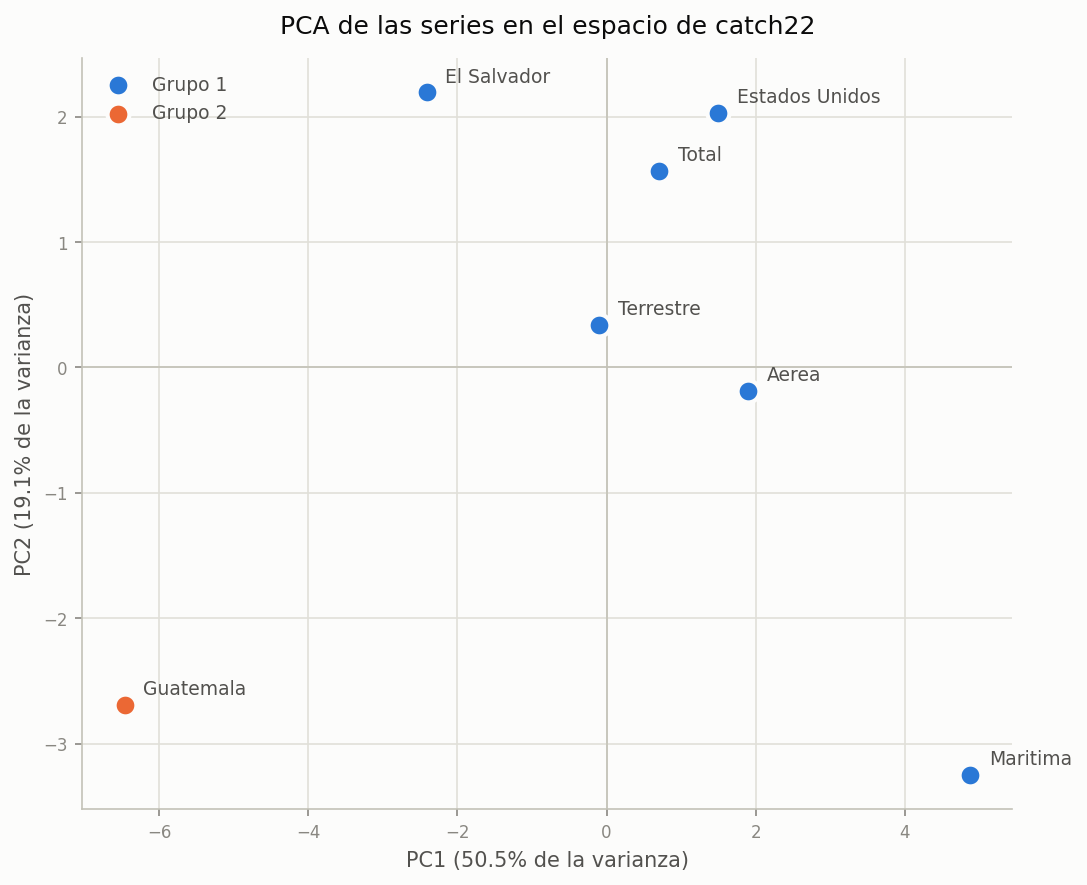
\includegraphics[width=0.75\textwidth]{results/Catch22Pca.png}
    \caption{Dispersión de las 7 series temporales en el plano de los dos primeros componentes principales (PC1 y PC2).}
    \label{fig:pca}
\end{figure}

\begin{figure}[H]
    \centering
    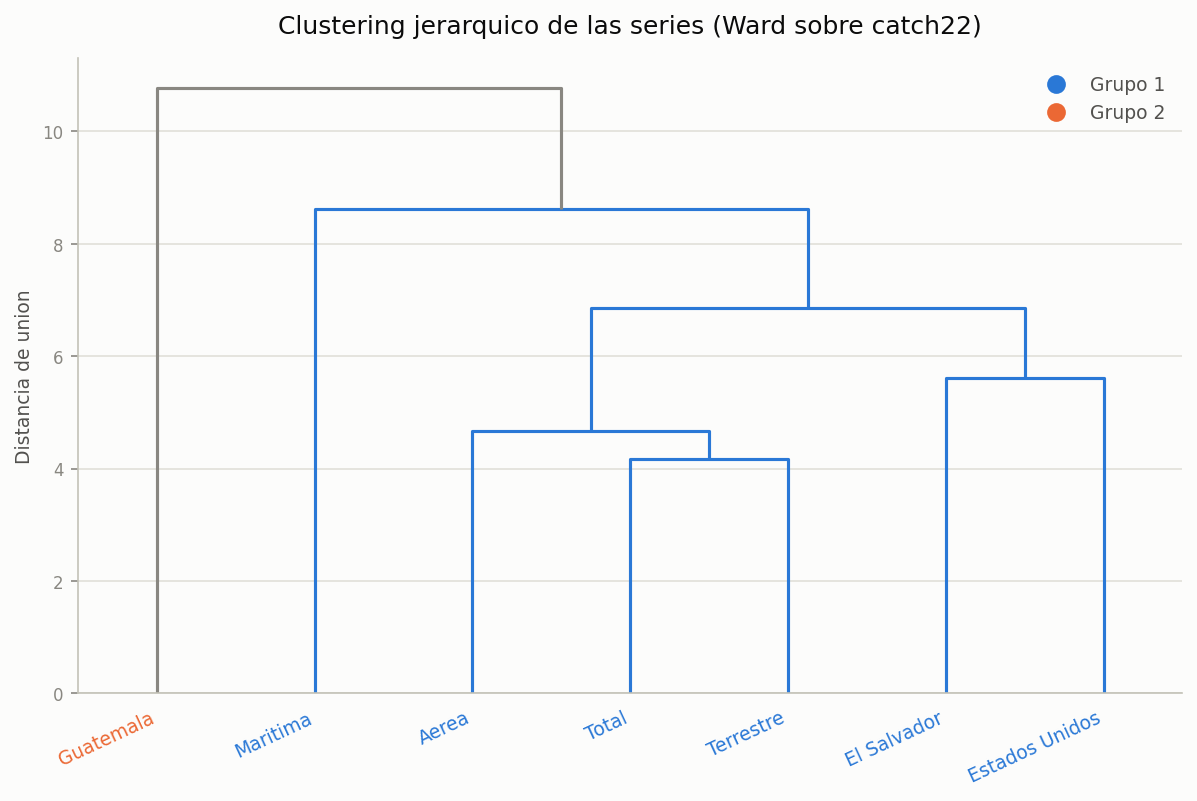
\includegraphics[width=0.85\textwidth]{results/Catch22Dendrograma.png}
    \caption{Dendrograma de clustering jerárquico usando el método de enlace de Ward sobre las características de catch22.}
    \label{fig:dendrograma}
\end{figure}

\begin{figure}[H]
    \centering
    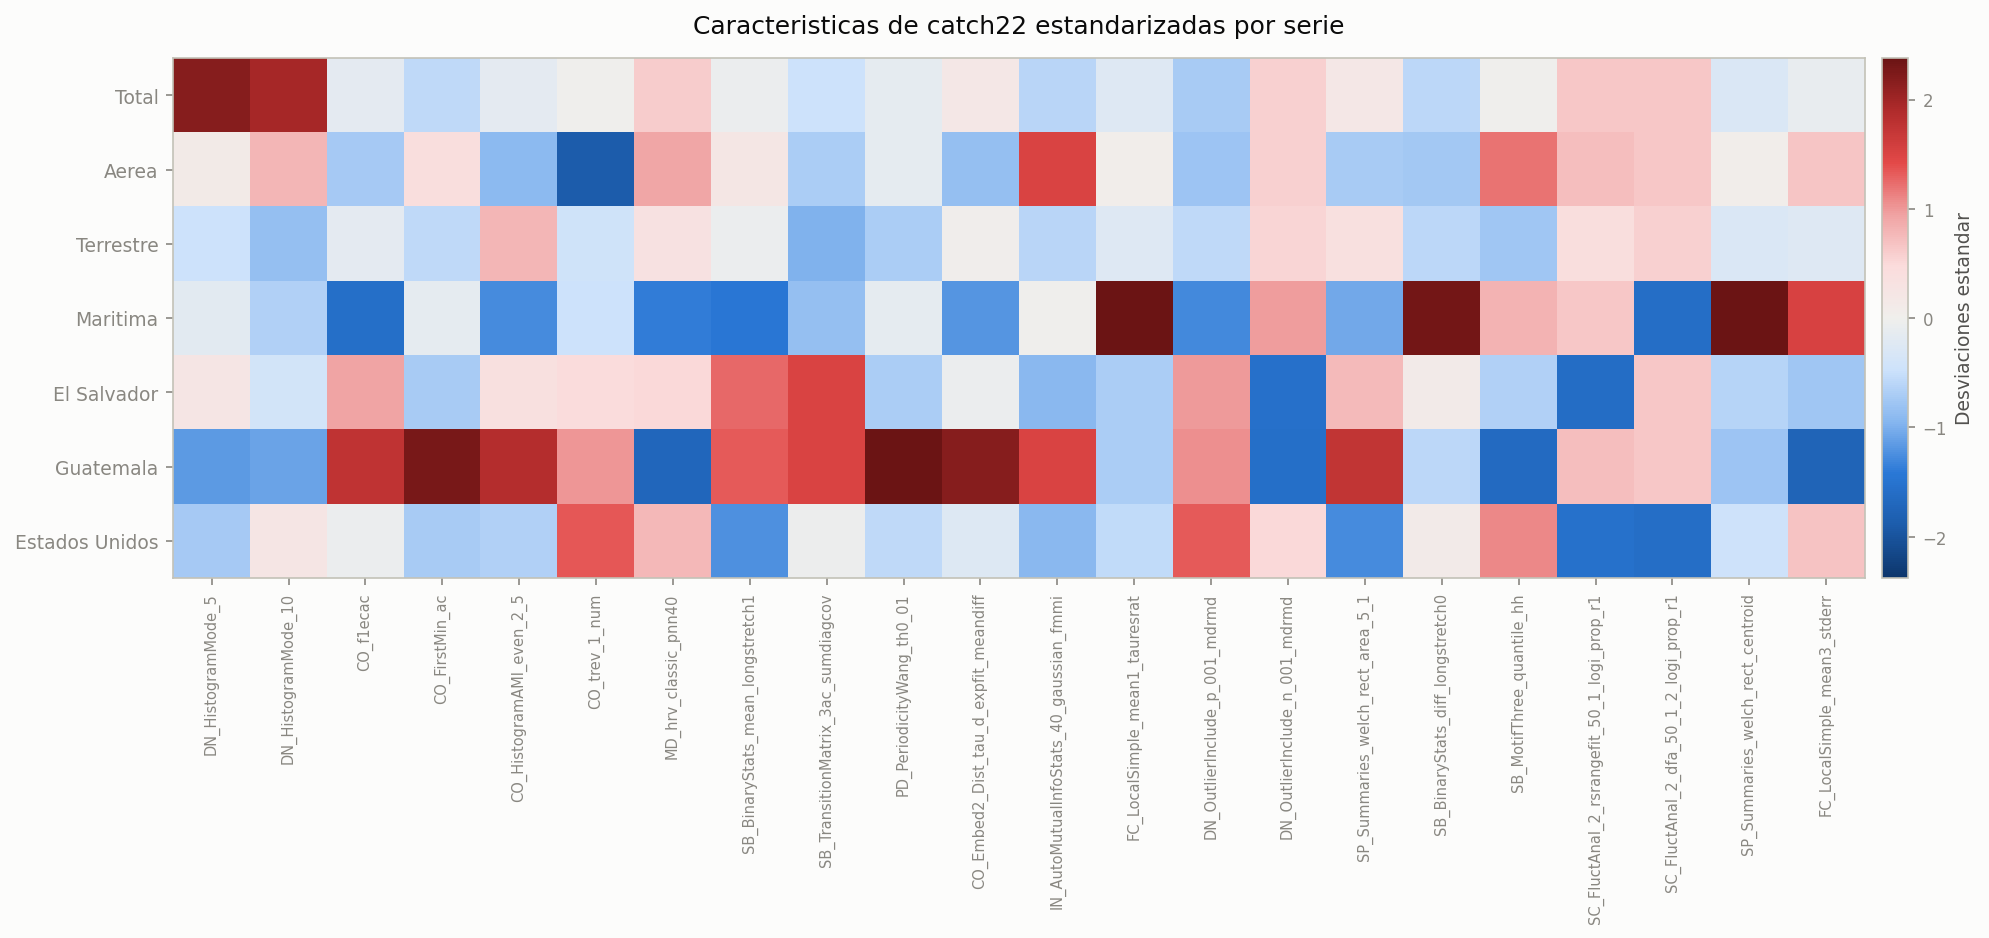
\includegraphics[width=0.95\textwidth]{results/Catch22Heatmap.png}
    \caption{Mapa de calor con las 22 características de catch22 estandarizadas para cada una de las 7 series.}
    \label{fig:heatmap}
\end{figure}

\begin{figure}[H]
    \centering
    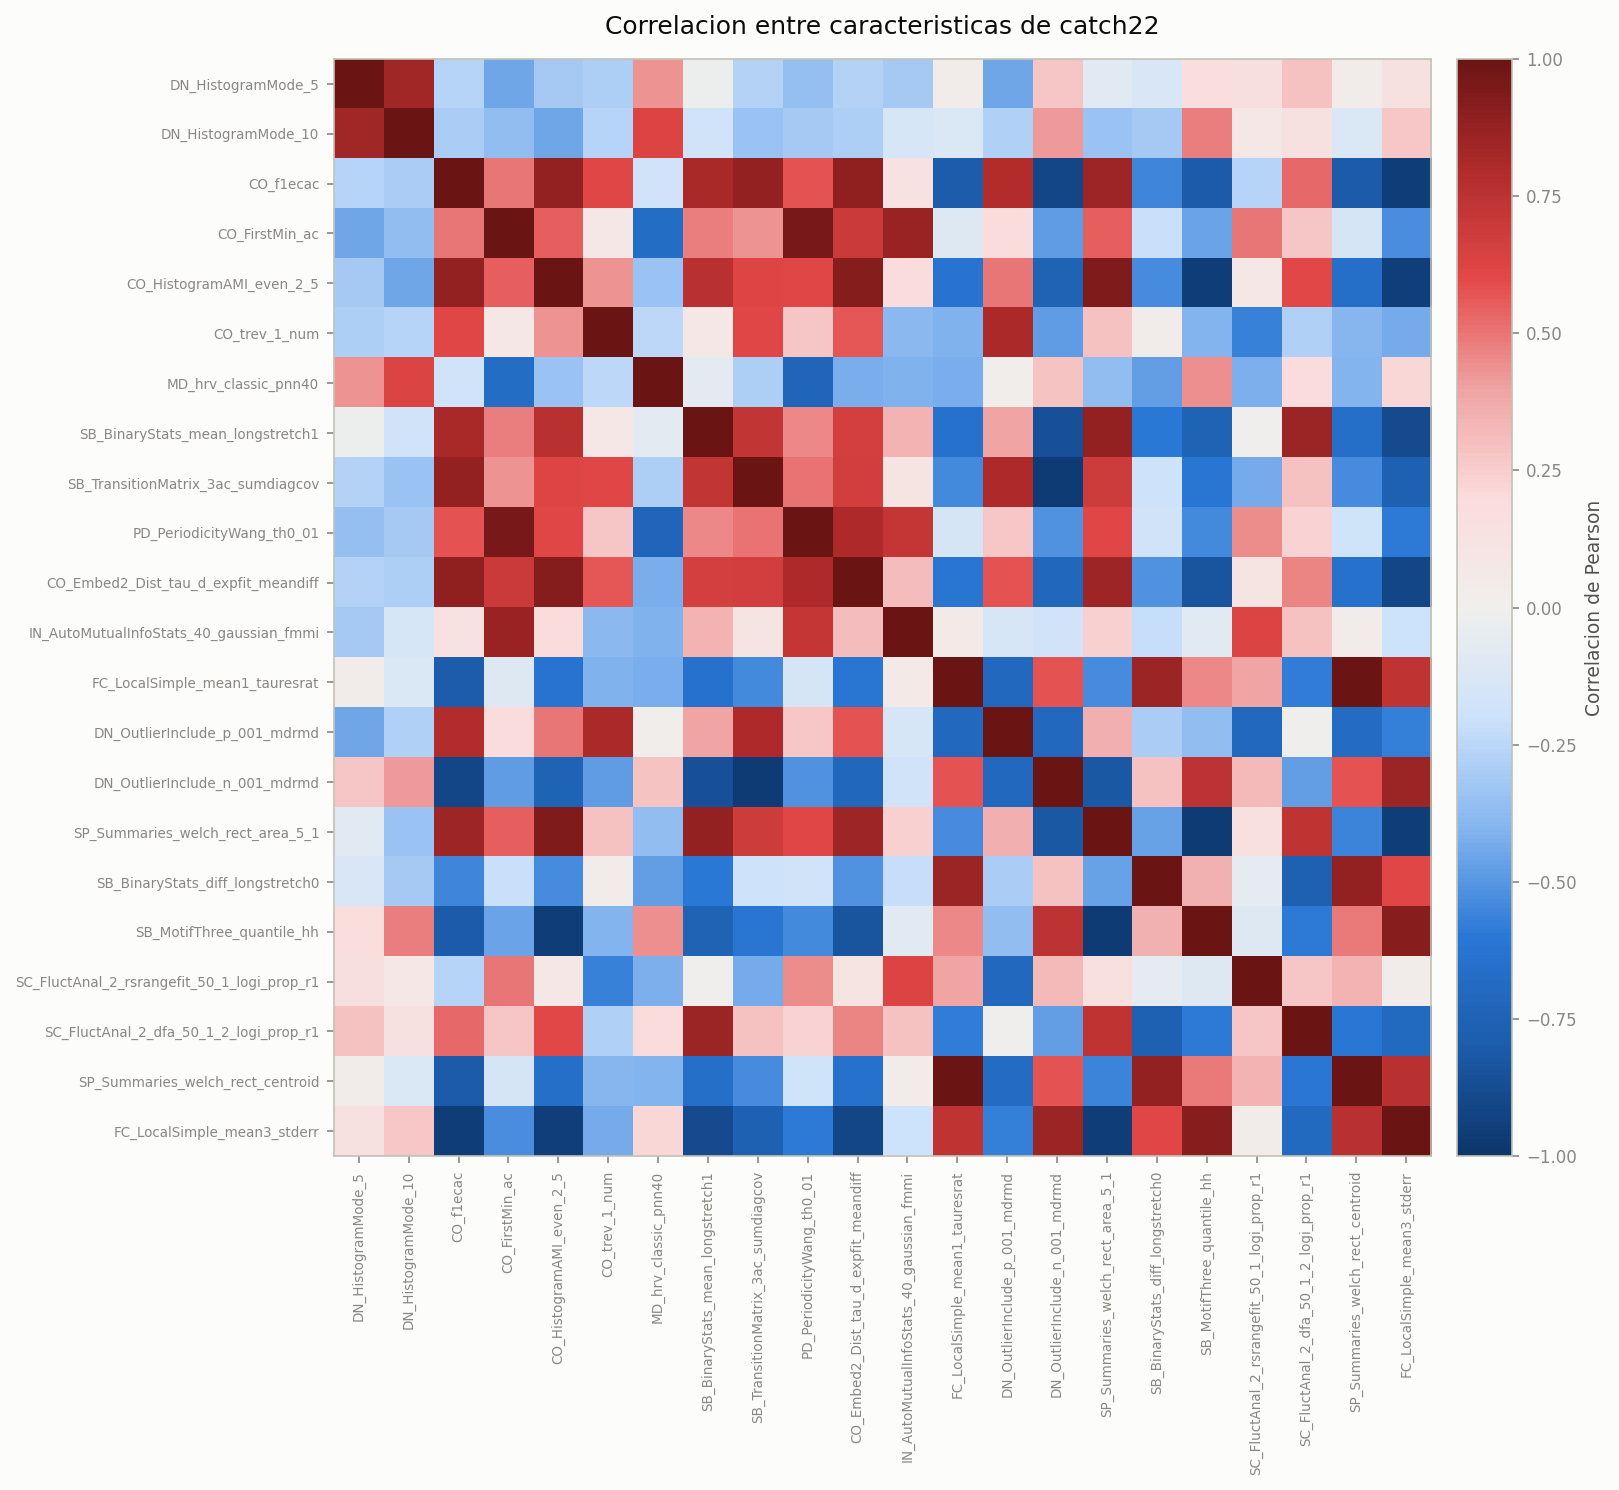
\includegraphics[width=0.8\textwidth]{results/Catch22Correlaciones.png}
    \caption{Matriz de correlaciones de Pearson entre las 22 características canónicas de catch22.}
    \label{fig:correlaciones}
\end{figure}

\begin{figure}[H]
    \centering
    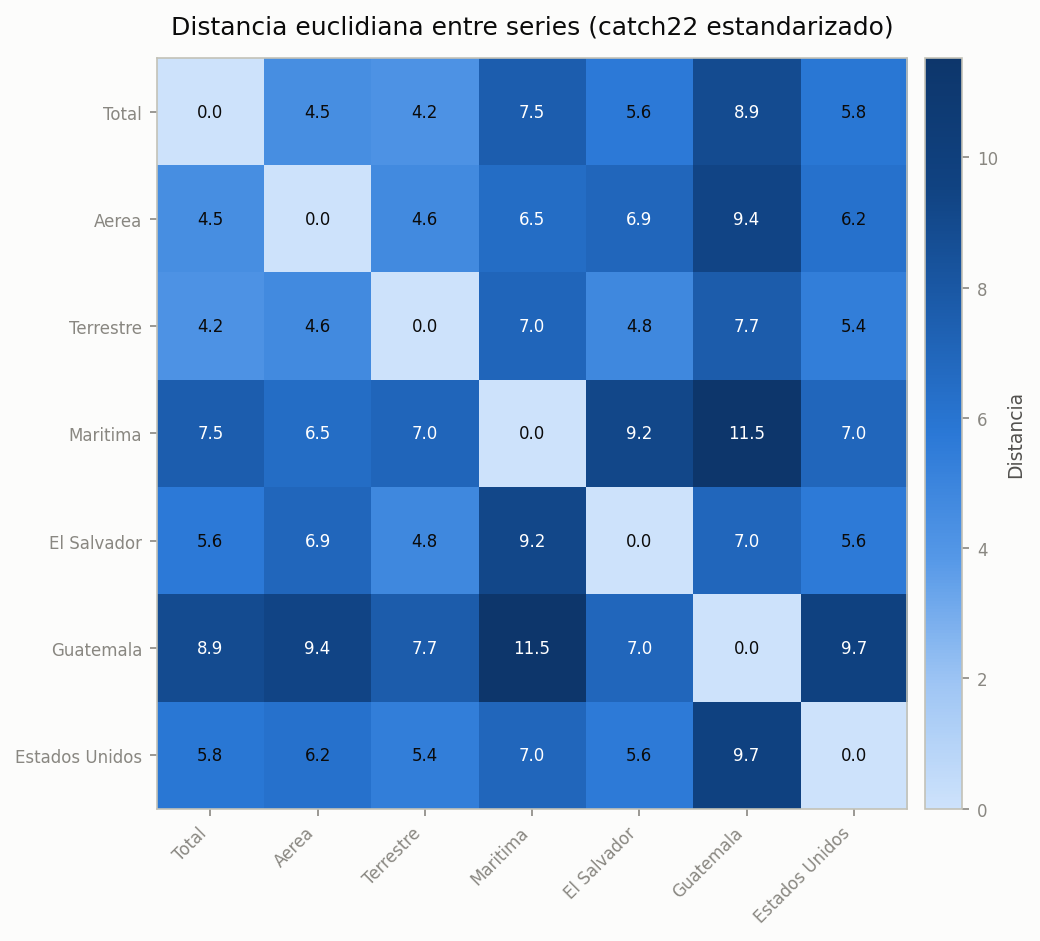
\includegraphics[width=0.75\textwidth]{results/Catch22Distancias.png}
    \caption{Mapa de distancias euclidianas par a par entre las series temporales estandarizadas.}
    \label{fig:distancias}
\end{figure}

\subsection{Análisis e Interpretación}

\subsubsection{¿Cuáles series presentan comportamientos más similares?}
Las series que exhiben el comportamiento dinámico más similar son \textbf{Total\_Consistent} y \textbf{Via\_Terrestre}, seguidas muy de cerca por \textbf{Pais\_El Salvador}. Esta afirmación se fundamenta cuantitativamente en tres hallazgos congruentes:
\begin{enumerate}
    \item \textbf{Distancia Euclidiana mínima:} En la matriz de distancias 22D, el par con menor distancia euclidiana de todo el estudio es $(\text{Total\_Consistent}, \text{Via\_Terrestre})$ con $d = 4.17$. Asimismo, Via\_Terrestre con Pais\_El Salvador registra $d = 4.81$, y Total\_Consistent con Via\_Aerea registra $d = 4.45$.
    \item \textbf{Agrupamiento en PCA:} En la proyección sobre el plano PC1--PC2, estas series se ubican fuertemente concentradas en el cuadrante negativo de PC1, compartiendo valores idénticos en parámetros de memoria lineal (\texttt{CO\_f1ecac}) e información mutua (\texttt{CO\_HistogramAMI\_even\_2\_5}).
    \item \textbf{Dendrograma de Clustering:} En el árbol de jerarquía, Total\_Consistent, Via\_Terrestre y Pais\_El Salvador se fusionan a la menor altura de distancia de unión, confirmando que comparten la misma estructura estacional y dinámica de transmisión temporal.
\end{enumerate}

\subsubsection{¿Qué características de catch22 fueron las más importantes para diferenciar las series?}
El análisis de cargas (\textit{loadings}) de los componentes principales determinó las características canónicas con mayor poder de discriminación:
\begin{itemize}
    \item \textbf{Primer Componente Principal (PC1 --- 50.5\% de varianza):}
    \begin{itemize}
        \item \texttt{FC\_LocalSimple\_mean3\_stderr} ($+0.2949$): Error de pronóstico local con media móvil de 3 puntos (mide la predictibilidad local de la serie).
        \item \texttt{CO\_f1ecac} ($-0.2937$): Retardo donde la autocorrelación cae por debajo de $1/e$ (mide la memoria temporal lineal).
        \item \texttt{CO\_HistogramAMI\_even\_2\_5} ($-0.2808$): Información mutua automática con retardo 2 (mide dependencias no lineales).
    \end{itemize}
    PC1 actúa como un eje de \emph{predictibilidad y memoria temporal}, separando series altamente estructuradas (como Total y Vía Terrestre) de series con quiebres o patrones irregulares.

    \item \textbf{Segundo Componente Principal (PC2 --- 19.1\% de varianza):}
    \begin{itemize}
        \item \texttt{MD\_hrv\_classic\_pnn40} ($+0.4295$): Proporción de diferencias sucesivas que superan $0.04$ desviaciones estándar (mide fluctuaciones rápidas o micro-volatilidad).
        \item \texttt{CO\_FirstMin\_ac} ($-0.3341$): Primer mínimo de la función de autocorrelación (mide la escala de la periodicidad/estacionalidad).
    \end{itemize}
    PC2 actúa como un eje de \emph{micro-volatilidad y escala estacional}, discriminando principalmente a \textbf{Via\_Maritima} debido a su régimen de variación mensual de alta frecuencia.
\end{itemize}

\subsubsection{¿Existen grupos naturales de series?}
La evaluación del coeficiente de silueta confirmó la presencia de $k = 2$ grupos naturales bien definidos:
\begin{itemize}
    \item \textbf{Grupo 1 (Grupo Macrodinámico / Principal):} Integrado por \texttt{Total\_Consistent}, \texttt{Via\_Aerea}, \texttt{Via\_Terrestre}, \texttt{Via\_Maritima}, \texttt{Pais\_El Salvador} y \texttt{Pais\_Estados Unidos}. Caracterizado por alta persistencia temporal, fuerte estacionalidad anual cíclica y un patrón de recuperación progresivo post-pandemia.
    \item \textbf{Grupo 2 (Grupo Atípico / Dislocado):} Conformado de manera aislada por \texttt{Pais\_Guatemala}. Esta serie se separa tempranamente en el dendrograma y se proyecta en el extremo positivo de PC1 debido a una racha inusualmente larga por encima de su media (\texttt{SB\_BinaryStats\_mean\_longstretch1}) y a un comportamiento dislocado respecto a los flujos turísticos internacionales estándar.
\end{itemize}

\end{document}